% Phase 3: Model Architecture
% Lead: Muhammad Hamid Abad

\section{Phase 3: Model Architecture and Formulation}

\subsection{Multi-Task Architecture Specification}
To satisfy both continuous distance regression and the auxiliary classification requirement,
we design a multi-task feed-forward neural architecture with 29-dimensional inputs:
\begin{itemize}
    \item \textbf{Input Layer}: 29 inputs comprising normalized coordinates $(x/N, y/N)$, goal-relative offsets $(dx/N, dy/N)$, and flattened $5 \times 5$ local obstacle window context.
    \item \textbf{Backbone Hidden Layers}: Three fully connected dense layers with dimensions $256 \to 256 \to 128$, equipped with ReLU non-linearities and dropout regularization ($p=0.10$).
    \item \textbf{Continuous Regression Head}: Linear output $(128 \to 1)$ predicting standardized distance $h^\ast/N$.
    \item \textbf{Auxiliary 10-Bin Classification Head}: Linear output $(128 \to 10)$ emitting unnormalized logits over distance deciles.
\end{itemize}

\begin{figure}[H]
    \centering
    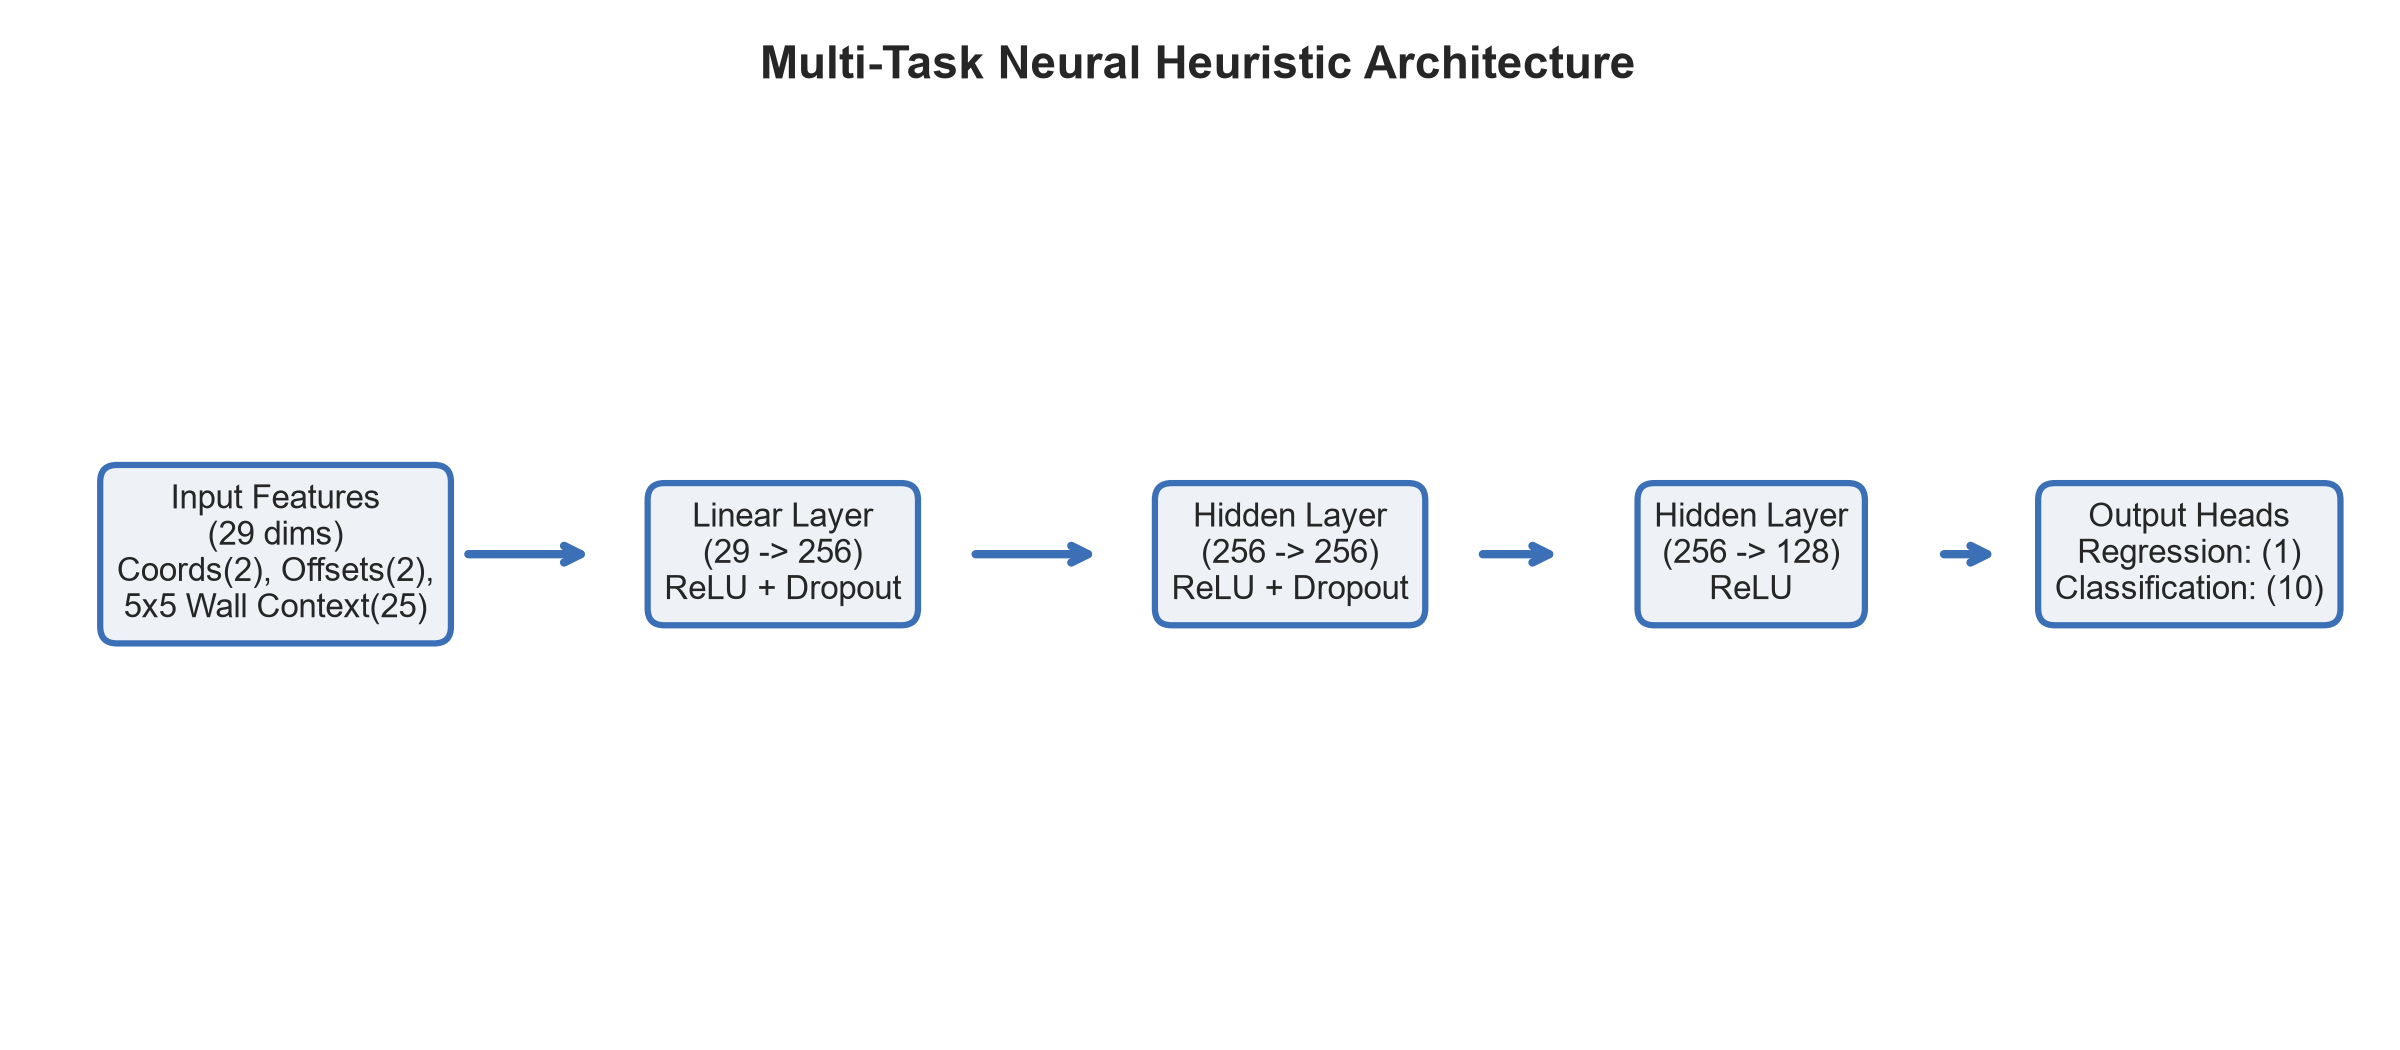
\includegraphics[width=0.88\textwidth]{figures/architecture.png}
    \caption{Multi-task neural heuristic network architecture with shared representation backbone.}
    \label{fig:model_architecture}
\end{figure}

\subsection{Heuristic Operational Modes}
During online graph search, predictions $\hat{h}_\theta(n)$ can be applied in three modes:
\begin{enumerate}
    \item \textbf{Raw}: Non-negatively clamped prediction $\max(0, \hat{h}_\theta(n))$.
    \item \textbf{Scaled}: Multiplied by scaling discount parameter $\alpha \in [0.6, 1.0]$ to enforce conservative admissibility.
    \item \textbf{Clipped Manhattan}: Upper-bounded by admissible Manhattan distance $\min(\alpha \hat{h}_\theta(n), h_{\text{man}}(n))$, ensuring provable admissibility and guaranteed path optimality.
\end{enumerate}
